\section{Verification of Algorithms}
In this section the implementation of Cov-DL and M-SBL are verified separately based on the MSE between the true and the estimated model parameters.
During the tests on simulated data sets the segmentation stage is ignored by letting the simulated data form one single segment.    

\subsection{Test of Cov-DL}
As seen from the flowchart \ref{fig:flow} Cov-DL takes a measurement matrix $\mathbf{Y}$, $N$ and $k$ as input and return an estimation $\hat{\mathbf{A}}$ of the mixing matrix $\mathbf{A}$. 
The Cov-DL algorithm is tested on the two simulations of the deterministic data, specified in section \ref{subseg_simpledata}. 

\subsubsection{Cov-DL1}
For $\mathbf{Y}$ specified by $N > \widetilde{M}$ and $k \leq \widetilde{M}$, implying Cov-DL1, the true and estimated values of $\mathbf{A}$ are plotted in figure \ref{fig:cov1_simple} for visual comparison. 
Note that each matrix is vectorized such that the corresponding entries are compared.  
The resulting $\text{MSE}(\mathbf{A}, \hat{\mathbf{A}})$ between the true $\mathbf{A}$ and the estimated $\hat{\mathbf{A}}$ become \todo{Jan vil gerne se på MSE(A, 0) også - L} 
\begin{align*}
\text{MSE}(\mathbf{A}, \hat{\mathbf{A}}) = 1.37.
\end{align*}
From figure \ref{fig:cov1_simple} it is seen that the precision of the estimate varies significant for each entry. 
Though, values within the a similar range are obtained.
Furthermore, the $\text{MSE}(\mathbf{A}, \hat{\mathbf{A}})$ is fairly small suggesting that the estimate is acceptable.


\subsubsection{Cov-DL2}
For $\mathbf{Y}$ specified by $N \leq \widetilde{M}$, implying Cov-DL2, the true and estimated values of $\mathbf{A}$ are plotted in figure \ref{fig:cov2_simple} for visual comparison. 
Additionally, is the initial $\mathbf{A}_{\text{ini}}$, given to the optimization solver within Cov-DL2, plotted in the same figure, as standard that is a Gaussian matrix. 
The resulting MSE between the true $\mathbf{A}$ and the estimated $\hat{\mathbf{A}}$ become 
\begin{align*}
\text{MSE}(\mathbf{A}, \hat{\mathbf{A}}) = 2.46.
\end{align*}
From figure \ref{fig:cov2_simple} the estimate $\hat{\mathbf{A}}$ shows visual tendencies from the true $\mathbf{A}$. 
However, when it is compared to the initial guess of $\textbf{A}$, $\mathbf{A}_{\text{ini}}$, it is observed that the estimate $\hat{\mathbf{A}}$ have moved further away from the true $\mathbf{A}$ compared to $\mathbf{A}_{\text{ini}}$. 
This suggests some flaw within the optimization process. 
By printing the convergence message from the used optimization solver, it is confirmed that the optimization process was found to be terminated successfully, with a current cost function value at $0.0$ after 26 iterations. 
This suggests that a global minimum has been found, but the minimum, $\hat{\mathbf{A}}$, do not correspond to the true $\mathbf{A}$. 
To confirm this the following evaluations of the cost function was conducted. 
\begin{align*}
&\text{cost}(\hat{\mathbf{A}}) = 0.0\\
&\text{cost}(\mathbf{A}_{\text{ini}}) = 1.564\\
&\text{cost}(\mathbf{A}) = 1.809
\end{align*}
These evaluations ensure that the optimization solver has managed to find the solution that minimizes the cost function. 
By evaluating the cost function with respect to the true $\mathbf{A}$ is it seen that it is not a global minimizer to the optimization problem. 
This suggests that the optimization problem, derived in section \ref{sec:over_det}, do not fulfil the purpose.
One reason for the optimization problem not fulfilling its purpose is that the cost function may no be convex. 
That is, in chapter \ref{ch:Cov-DL} it was assumed that the cost function was convex but no further investigate regarding the truthfulness of this assumption was made. As this was not possible to do \todo{Tjek dette afsnit omkring hvorfor optimisering problem ikke lykkes, cost funktion værende non-convex}.
\begin{figure}[H]
    \begin{minipage}[t]{.45\textwidth}
		\centering
		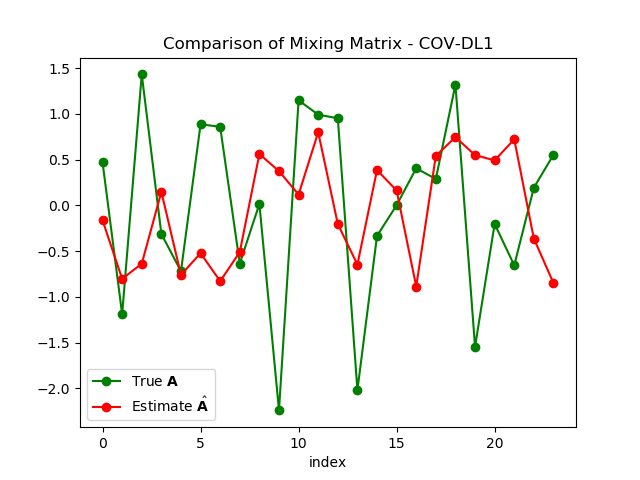
\includegraphics[scale=0.5]{figures/ch_6/COV1_simple.png}
		\caption{Estimated values of $\hat{\mathbf{A}}$ compared to the true 				values $\mathbf{A}$}
		\label{fig:cov1_simple}
    \end{minipage} 
    \hfill
    \begin{minipage}[t]{.45\textwidth}
        \centering
		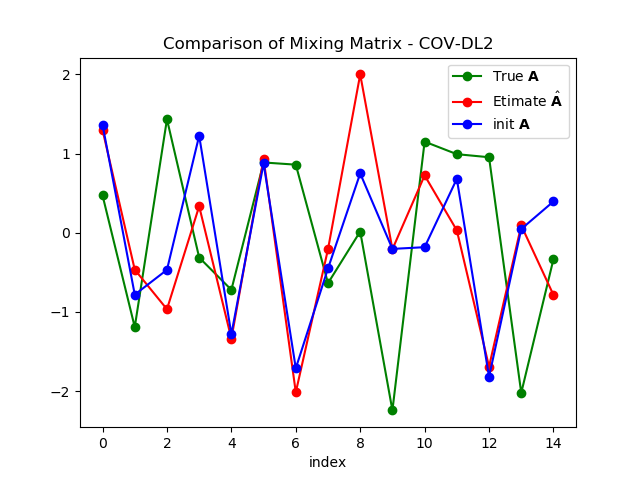
\includegraphics[scale=0.5]{figures/ch_6/COV2_simple.png}
		\caption{The initial $\mathbf{A}_{\text{ini}}$ and the estimate $\hat{\mathbf{A}}$ 				compared to the true values $\mathbf{A}$. }
		\label{fig:cov2_simple}
    \end{minipage}
\end{figure}

\subsubsection{Conclusion to Estimate $\hat{\mathbf{A}}$}
From the results of the evaluation of cost function it is found that the estimate $\hat{\mathbf{A}}$, especially within the Cov-DL2 branch, can not be consider a valid estimate of the mixing matrix $\mathbf{A}$. 
It is suggested that the flaw lies within either the  derivation of the cost function to the optimization problem, more specifically within the assumption made throughout the derivation concerning the relation between $\mathbf{A}, \mathbf{D}$ and $\mathbf{U}$. 
This statement build upon the success of the (non-documented) unit tests of the Cov-DL2 algorithm suggesting that the optimization of $\mathbf{D}$ not depending on $\mathbf{A}$ is possible.
The appearance of this issue may suggest that there is a lack within the published results \cite{Balkan2015} considering the possibility of reproducibility of the results.  

Due to the time limitation of the project the error is not investigated further, and it is concluded that the estimate of $\mathbf{A}$ is not valid hence it will not be used as an input for the next stage of the main algorithm, M-SBL. This conclusion suggest that an alternative action must be considered. This is discussed further in section \ref{sec:test_base}.

\subsection{Test of M-SBL}
From the flowchart \ref{fig:flow} it seen that the M-SBL algorithm takes $\hat{\mathbf{A}}$ and $\mathbf{Y}$ as input.
The algorithm is first tested on a deterministic data set specified by $M=N=k=4$ and $L=100$. This result will serve as a reference, showing the best possible performance due to the system having equal number of equations and unknowns, hence a unique solution exist.
In order to not let the performance of Cov-DL affect the result of M-SBL the true mixing matrix $\mathbf{A}$ is used as input through out this section, along with the corresponding $\mathbf{Y}$. 
The resulting estimate is seen in figure \ref{fig:M-SBL_simple0}. It is seen that the source signals is estimated exact, with $MSE(\textbf{X},\hat{\textbf{X}})= 0$. 
\begin{figure}[H]
\centering
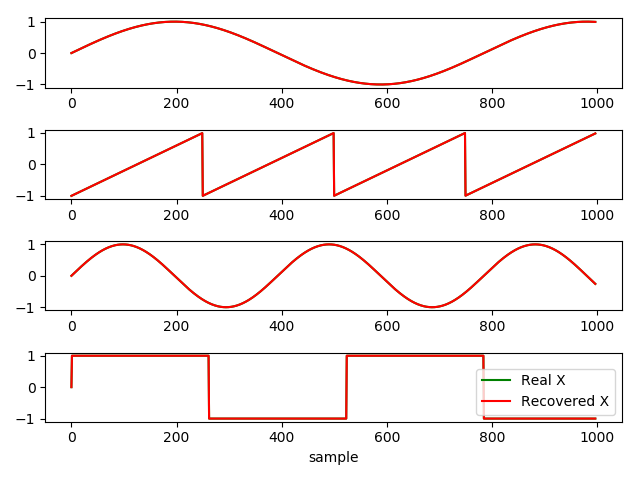
\includegraphics[scale=0.5]{figures/ch_6/M-SBL_simple0.png}
\caption{Estimated values of $\hat{\textbf{X}}$ compared to the true values $\textbf{X}$. From deterministic data $\textbf{Y}$ specified by $N=k=4$, $M = 3$ and $L=1000$}
\label{fig:M-SBL_simple0}
\end{figure}

Now the desired case of $M<N$ is considered. Two tests is performed on the same two deterministic data sets, as used in the previous section, specified by $M = 3$, $k = 4$, $L=1000$ and respectively $N = 5$ and $N = 8$.

The estimate $\hat{\mathbf{X}}$ is plotted in figure \ref{fig:M-SBL_simple1} and \ref{fig:M-SBL_simple2}. The source signals equal to zeros of the estimate $\hat{\mathbf{X}}$ is not plotted so the figures do not visualize the exact localization of the source signals.
%Each non-zero signals are here plotted separately for easy visual comparison. 
%Furthermore, note that each compared couple of rows have the same row index, as such the localization of the estimated row can be evaluated.
\begin{figure}[H]
    \begin{minipage}[t]{.45\textwidth}
    	\centering
		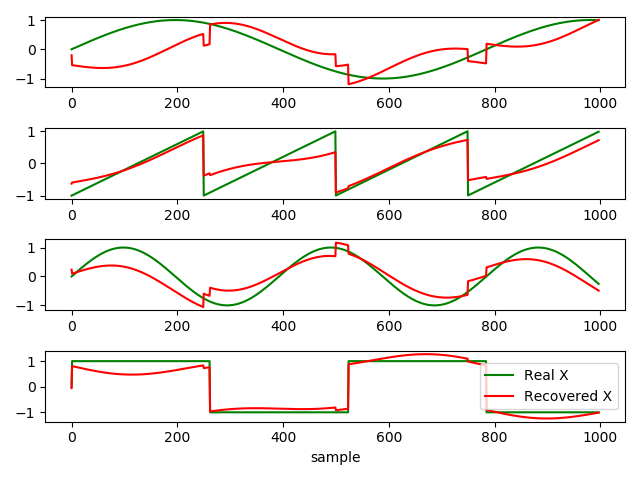
\includegraphics[scale=0.45]{figures/ch_6/M-SBL_simple1.png}
		\caption{Estimated values of $\hat{\mathbf{X}}$ compared to the true 					values $\mathbf{X}$. From measurement $\mathbf{Y}$ specified by $N=5$, $M = 3$, $k=4$ and $L=1000$ and the true mixing matrix $\mathbf{A}$.}
		\label{fig:M-SBL_simple1}
    \end{minipage} 
    \hfill
    \begin{minipage}[t]{.45\textwidth}
        \centering
		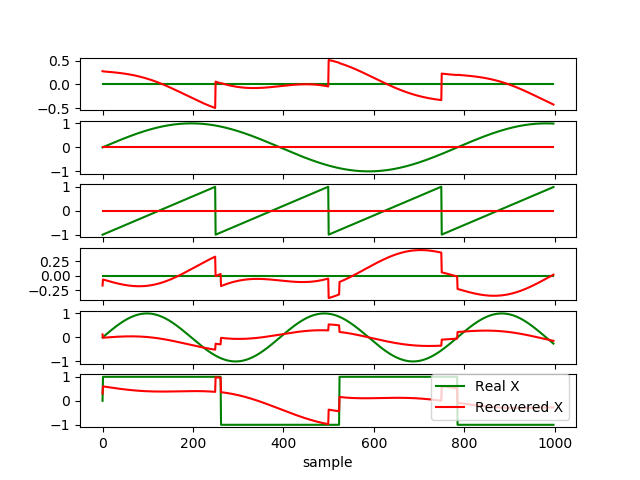
\includegraphics[scale=0.45]{figures/ch_6/M-SBL_simple2.png}
		\caption{Estimated values of $\hat{\mathbf{X}}$ compared to the true values $\mathbf{X}$. From measurement $\mathbf{Y}$ specified by $N=8$, $M = 3$, $k=4$ and $L=1000$ and the true mixing matrix $\mathbf{A}$.}
		\label{fig:M-SBL_simple2}
    \end{minipage}
\end{figure}
\noindent
The resulting MSE between the true $\mathbf{X}$ and the estimate $\hat{\mathbf{X}}$ from figure \ref{fig:M-SBL_simple1} with $N = 5$, becomes 
\begin{align*}
\text{MSE}(\mathbf{X}, \hat{\mathbf{X}}) = 0.127.
\end{align*}
From figure \ref{fig:M-SBL_simple1} it is seen that all four source signals are recovered at the right locations. 
As suggested by the achieved MSE the estimate is not exact, but it is clear that the estimates, by looking at figure \ref{fig:M-SBL_simple1}, manage to follow the right pattern of the true signals. 

The resulting MSE between the true $\mathbf{X}$ and the estimated $\hat{\mathbf{X}}$ from figure \ref{fig:M-SBL_simple2} with $N = 8$ thus more sparse, become 
\begin{align*}
\text{MSE}(\mathbf{X}, \hat{\mathbf{X}}) = 0.161. 
\end{align*}
From figure \ref{fig:M-SBL_simple2} it is again seen that the source signals are recovered at the right location. However visually the estimates are not as .  
%From figure \ref{fig:M-SBL_simple2} it is seen that the first source signal is recovered at the third entry, that is one dislocation, while the rest are recovered at the right locations. 
This indicate that the algorithm can manage to locate and estimate the source signals, however the increased zero rows improve the chance of dislocation and the decrease the accuracy of the estimate.     

\subsubsection*{Possibilities of $N=k$}

From the problem statement in chapter \ref{ch:problemstatement} it is an issue that $k$ has to be known a prior, in order to estimate $\textbf{A}$ and $\textbf{X}$. A short discussion in subsection \ref{subsec:kestimate}, describes how k can be estimated within the M-SBL algorithm. However one still needs to provide k in order to estimate $\textbf{A}$, thus an qualified estimate of k can not be avoided. 

Similar to k, the maximum number of active sources $N$ is unknown in practise as it is described in chapter \ref{ch:motivation}. 
The difference between $k$ and $N$ defines the number of zero rows in $\textbf{X}$.
During the estimation of $\textbf{X}$ the localisation of the non-zero rows are in general significant to minimize the MSE. However, the fact that the true $N$ can not be known for EEG measurements weakens the argument for of focusing on the localisation rather than only focusing on the value estimation of the source signals. Furthermore it is not within the main scope of this thesis to localise the source signal.  
When considering the linear system, $\textbf{Y}=\textbf{AX}$, of which the model is build, $\textbf{Y}$ does not change by removing the zero-rows of $\textbf{X}$ and the corresponding columns in $\textbf{A}$.
 
From this is can be argued that letting $N = k$ is as good an estimate of $N$ as any other. Note in order to fulfil the sufficient conditions for the existence of a solution to the system, that $k$ hence $N$ is limited by $\widetilde{M}$ \todo{ "as any other" - forsøg at omformulere, alernativt er det bare et valg vi tager ud den begrundelse}.     

Consider the effect of letting $N = k$ within the M-SBL algorithm. Here it is only the estimation of the support set which is eliminated.   

Figure \ref{fig:M-SBL_simple3} show the estimated sources signal for a simulation of the deterministic data set now specified by $N=k=4$ $M = 3$ and $L=1000$. The resulting MSE become
\begin{align*}
\textbf{X}_{MSE} = 0.121
\end{align*}

\begin{figure}[H]
\centering
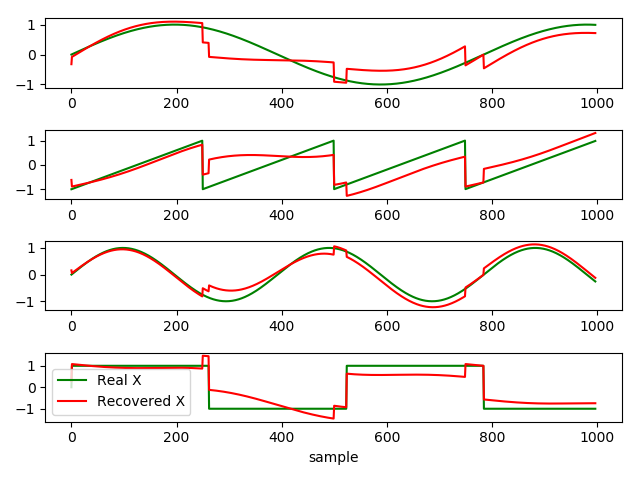
\includegraphics[scale=0.5]{figures/ch_6/M-SBL_simple3.png}
\caption{Estimated values of $\hat{\textbf{X}}$ compared to the true 				values $\textbf{X}$. From deterministic data $\textbf{Y}$ specified by $N=k=4$, $M = 3$ and $L=1000$ }
\label{fig:M-SBL_simple3}
\end{figure}

From the above discussion and the results in figure \ref{fig:M-SBL_simple3} it is confirmed that letting $N=k$ has no disadvantage with respect to the results, when the localisation of the source signal is not a priority. Thus is it chosen that $N=k$ will be used throughout the thesis. 

\subsection{Test on Stochastic Data Sets}\label{sec:testMsbl_stoch}
The M-SBL algorithm is now tested on two stochastic data sets which resembles the real EEG measurements. 
The first stochastic data set is simulated with specification $N=k=8$, $M = 6$, $L=1000$. 
The resulting estimate is plotted in figure \ref{fig:AR1} and the MSE becomes 
\begin{align*}
\text{MSE}(\mathbf{X}, \hat{\mathbf{X}}) = 1.643.
\end{align*}  
The second stochastic data set is simulated with specification $N=k=16$, $M = 6$, $L=1000$. 
This tests the capabilities of the M-SBL algorithm when the distance between $M$ and $N$ is enlarged. 
The performance relative to the relation between $N$ and $M$ is further investigated for the main algorithm in section \ref{sec:test_base}.
The resulting estimate is plotted in figure \ref{fig:AR2} and the MSE becomes 
\begin{align*}
\text{MSE}(\mathbf{X}, \hat{\mathbf{X}}) = 5.182. 
\end{align*}  

\begin{figure}[H]
    \begin{minipage}[t]{.45\textwidth}
    	\centering
		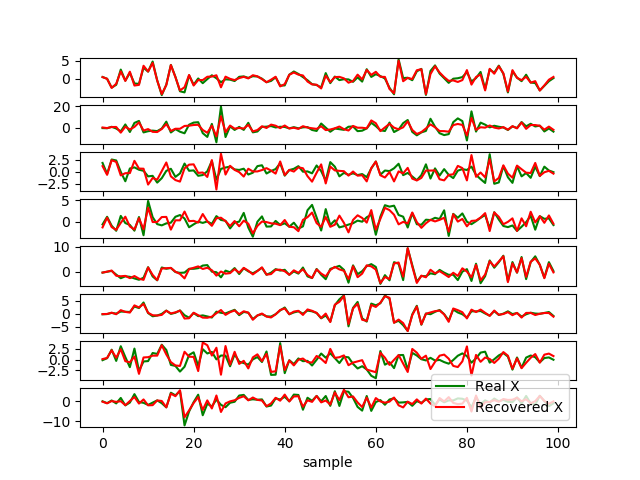
\includegraphics[scale=0.5]{figures/ch_6/M-SBL_AR1.png}
		\caption{Estimated values of $\hat{\mathbf{X}}$ compared to the true 					values $\mathbf{X}$. From measurement $\mathbf{Y}$ specified by $N=k=8$, $M = 6$ and $L=1000$ and the true mixing matrix $\mathbf{A}$}
		\label{fig:AR1}
    \end{minipage} 
    \hfill
    \begin{minipage}[t]{.45\textwidth}
        \centering
		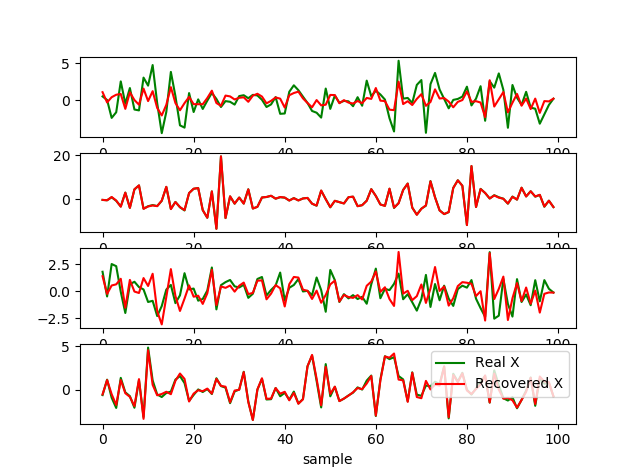
\includegraphics[scale=0.5]{figures/ch_6/M-SBL_AR2.png}
		\caption{Estimated values of $\hat{\mathbf{X}}$ compared to the true 					values $\mathbf{X}$. From measurement $\mathbf{Y}$ specified by $N=k=16$ $M = 6$ and $L=1000$ and the true mixing matrix $\mathbf{A}$}
		\label{fig:AR2}
    \end{minipage}
\end{figure}
\noindent
From figure \ref{fig:AR1} it is visually confirmed that the M-SBL algorithm manage to recover the source signals of the source matrix $\mathbf{X}$. 
Some source signals nearly perfect estimated while other are have minor differences. 
From figure \ref{fig:AR2} the same tendency is seen, though more visual flaws are seen compared to figure \ref{fig:AR1}. 
This result suggest that a bigger distance between $M$ and $N$ results in a worse performance from the M-SBL algorithm.        

%\subsection{Model Fitting}
Two model variables are now considered with the purpose of improving the performance of the COV-DL algorithm. The initial A given to the optimization problem \eqref{eq:Cov_DL2} within COV-DL2, and the segmentation size used within the covariance domain.   
\subsubsection*{Initial $\textbf{A}$}
Consider the COV-DL algorithm in the case where the system transformed into the covariance domain results in an overdetermined system. In this case the COV-DL2 branch of the algorithm is used. 
When estimating the mixing matrix $\mathbf{A}$ a matrix $\mathbf{D}$ is used in the process. For the over-determined system \ref{sec:over_det} $\mathbf{D}$ is found by solving the optimisation problem \eqref{eq:Cov_DL2} with respect to $\hat{\textbf{A}}$. To solve the optimization problem an initial $\mathbf{A}_{\text{ini}}$ is given. The choice of this initial $\mathbf{A}_{\text{ini}}$ may affect how the good an estimate the recovered mixing matrix $\mathbf{A}$ is.
Three different choices of $\mathbf{A}_{\text{ini}}$ are considered:
\begin{itemize}
\item[-] A matrix $\mathbf{A1}$ drawn from a continuous uniform distribution in the half-open interval $[0.0, 1.0)$
\item[-] A matrix $\mathbf{A2}$ drawn from a uniform distribution in the half-open interval $[-1.0, 1.0)$
\item[-] A matrix $\mathbf{A3}$ drawn from a Gaussian distribution with mean 0 and variance 1
\end{itemize}
The test of different initial $\mathbf{A}_{\text{ini}}$ is performed on the 
an AR data set specified by $N=5$ $M = 3$, $k = 4$ and $L = 1000$. 
The MSE of the three tests are seen in table \ref{tab:iniA} 
\begin{table}[H]
\centering
\begin{tabular}{|l|l|l|l|} 
\hline
                          & \textbf{A1} & \textbf{A2} & \textbf{A3} \\
\hline $\text{MSE}_{\mathbf{A}}$ &   2.15          & 2.00            & 1.88\\
\hline           
\end{tabular}
\caption{Resulting MSE for varying initial A, used within COV-DL2.}
\label{tab:iniA}
\end{table}
\todo[inline]{is it okay that we do not include the mse of X here, I don't think is any reasoning to do it, but it should be check later whether the error of A follows the error of X as it is asumped at this moment.}
From the results it is seen that \textbf{A3} achieves the lowest MSE, thus an Gaussian distributed initial $\textbf{A}$ will be used.    
 






 
